% Problem 3 publication-figure snippets (A-route Final canonical 数据)。
% 时间口径统一 H-END：slot 1 = 0:00-0:10 … slot 144 = 23:50-24:00，横轴为物理时刻 0-24 h。
% 正文图：P3-1 ~ P3-10；技术路线图：fig_roadmap。
% 配色与版式对齐 P1 / P2：tol_vibrant、Times New Roman + SimSun、白底去上右边框。

% ---- 正文图 ----
\begin{figure}[htbp]
  \centering
  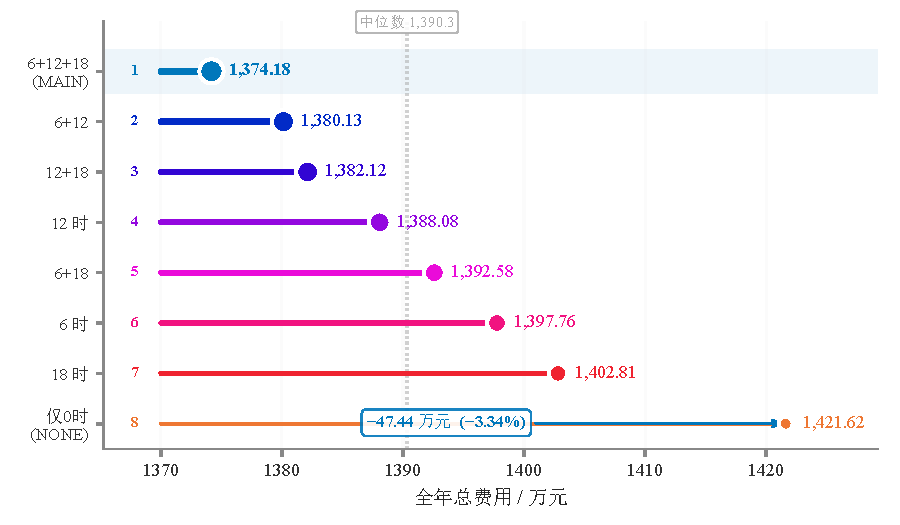
\includegraphics[width=0.85\textwidth]{figures/fig_p3_opportunity.pdf}
  \caption{8 种更新时间机会组合下的全年总费用。仅 0 时不调整约 1421.62 万元；依次开放 6/12/18 滚动更新后，MAIN 方案降至 1374.18 万元，节省约 47.44 万元（3.34\%）。点越靠左费用越低，横轴自 1370 万元起截断以放大差异；不得把单节点差额直接相加。数据源：\texttt{data/p3\_opportunity\_comparison.csv}（334 天正式期）。}
  \label{fig:p3-opportunity}
\end{figure}

\begin{figure}[htbp]
  \centering
  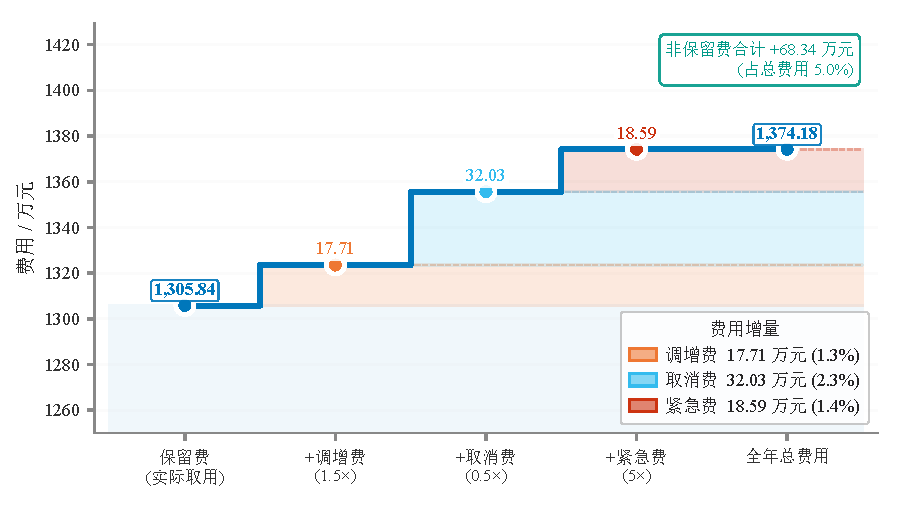
\includegraphics[width=0.85\textwidth]{figures/fig_p3_cost_structure.pdf}
  \caption{MAIN 全年费用结构分解。保留费 1305.84 万元（占 95.0\%）为账单主体，其上依次叠加调增费 17.71 万元、取消费 32.03 万元与紧急费 18.59 万元，合计全年总费用 1374.18 万元；非保留费合计仅占 5.0\%，说明费用风险主要来自合同调整而非紧急购电。数据源：\texttt{data/FINAL\_KEY\_RESULTS.csv}。}
  \label{fig:p3-cost-structure}
\end{figure}

\begin{figure}[htbp]
  \centering
  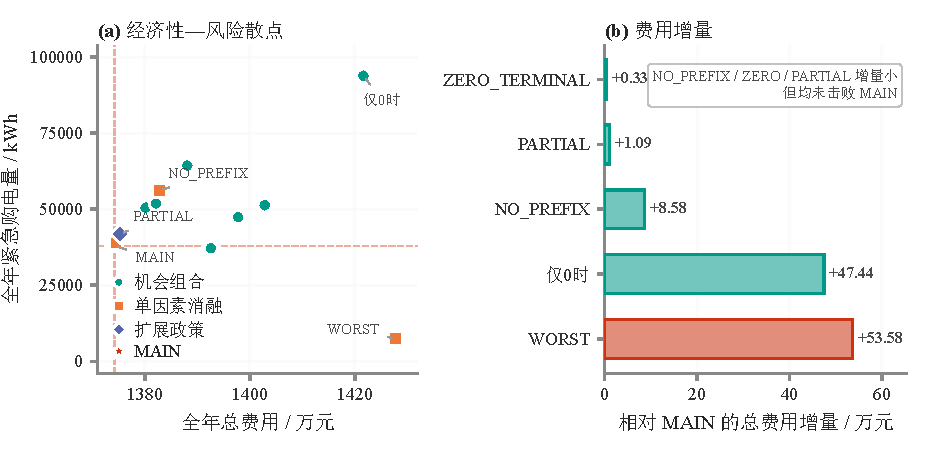
\includegraphics[width=0.85\textwidth]{figures/fig_p3_cost_risk.pdf}
  \caption{政策的经济性—风险权衡。(a) 横轴全年总费用、纵轴全年紧急购电量：WORST 把紧急购电量压到 7\,489 kWh（较 MAIN 低 80.3\%），但总费用升至 1427.76 万元（$+53.58$ 万元），落在费用最高处；(b) 相对 MAIN 的费用增量显示 ZERO\_TERMINAL（$+0.33$）、PARTIAL（$+1.09$）、NO\_PREFIX（$+8.58$）、仅0时（$+47.44$）均高于 MAIN。数据源：\texttt{data/p3\_cost\_risk\_tradeoff.csv}。}
  \label{fig:p3-cost-risk}
\end{figure}

\begin{figure}[htbp]
  \centering
  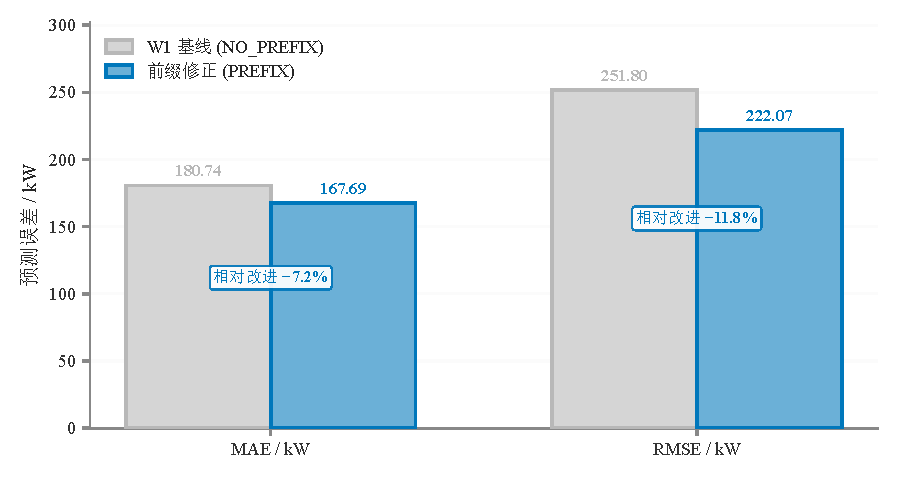
\includegraphics[width=0.85\textwidth]{figures/fig_p3_forecast_prefix.pdf}
  \caption{负荷预测精度对照。纯 W1 基线（NO\_PREFIX）的负荷 MAE/RMSE 为 180.74/251.80 kW，叠加当天已观测前缀的低维收缩修正（PREFIX）后降至 167.69/222.07 kW，相对改进 7.2\%/11.8\%。样本为发行—目标重叠记录（77\,328 条），不是独立盲测，仅用于说明前缀修正的贡献。数据源：\texttt{data/p3\_forecast\_prefix\_summary.csv}。}
  \label{fig:p3-forecast-prefix}
\end{figure}

\begin{figure}[htbp]
  \centering
  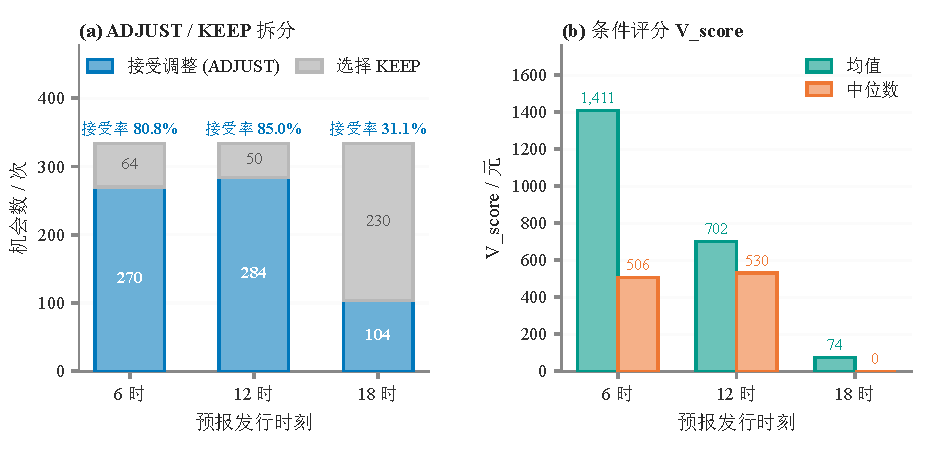
\includegraphics[width=0.85\textwidth]{figures/fig_p3_adjustment.pdf}
  \caption{6/12/18 时的合同调整执行率与 KEEP 决策。(a) 每个发行时刻 334 次机会中，6 时接受 270 次、12 时接受 284 次、18 时仅接受 104 次，对应接受率 80.8\%/85.0\%/31.1\%；全年 1002 次机会共执行 658 次修改、KEEP 344 次。(b) 条件评分 V\_score 的均值/中位数随发行时刻递减，18 时中位数近 0，说明新预报到达不等于必须调整。数据源：\texttt{data/p3\_adjustment\_issue\_summary.csv}。}
  \label{fig:p3-adjustment}
\end{figure}

\begin{figure}[htbp]
  \centering
  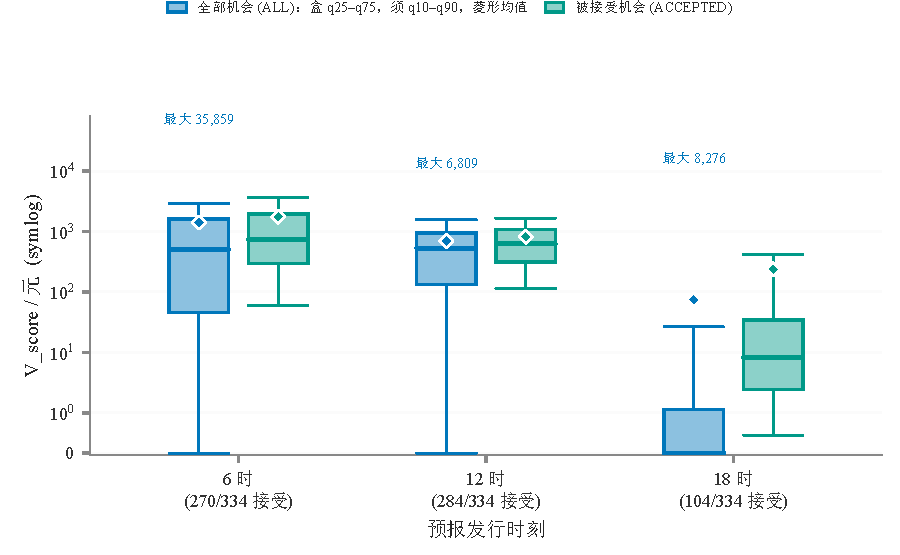
\includegraphics[width=0.85\textwidth]{figures/fig_p3_vscore.pdf}
  \caption{各发行时刻 $V_{\mathrm{score}}=\text{keep}-\text{selected}$ 的分布。盒为 q25--q75、须为 q10--q90、菱形为均值；6/12 时分布明显为正（中位数 506/530 元），18 时中位数约为 0，被拒节点 $V_{\mathrm{score}}$ 恒为 0，表明多数 18 时机会不值得改动计划。纵轴用 symlog 兼容 0 与小量级；数据为分位数汇总而非原始逐点。数据源：\texttt{data/p3\_vscore\_summary.csv}。}
  \label{fig:p3-vscore}
\end{figure}

\begin{figure}[htbp]
  \centering
  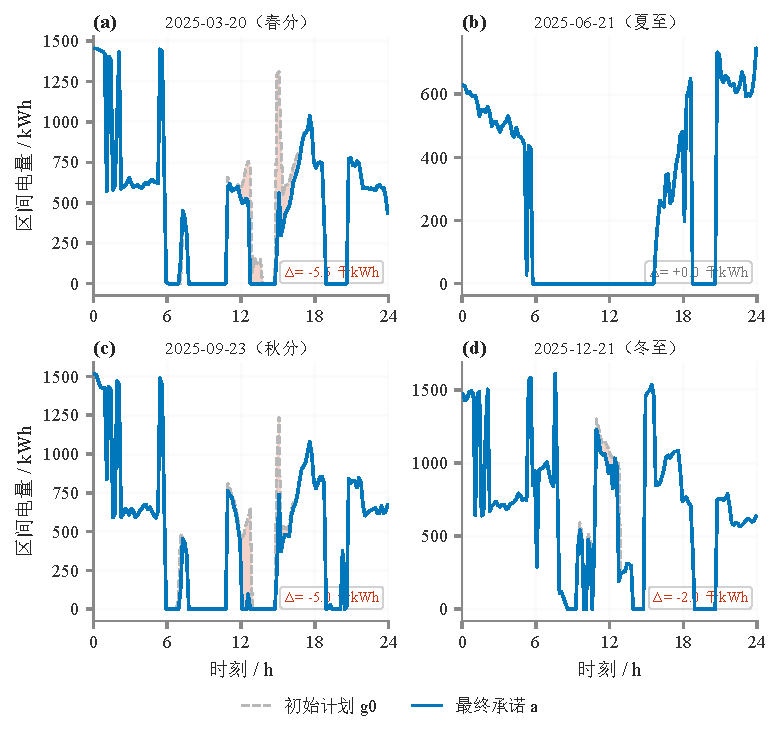
\includegraphics[width=0.70\textwidth]{figures/fig_p3_specified_purchase.pdf}
  \caption{四个指定日的初始计划 $g^0$ 与最终承诺 $a$。2025-03-20 与 2025-09-23 出现调整（$\Delta$ 分别为 $-5.5$、$-5.0$ 千kWh），调整集中于白天时段；2025-06-21、2025-12-21 无调整（$\Delta\approx 0$），18 时后承诺基本冻结。阴影为 $a$ 与 $g^0$ 之差（调减/取消）。数据源：\texttt{data/p3\_specified\_dates\_timeseries.csv}（144 槽/日，区间电量 kWh/10min）。}
  \label{fig:p3-specified-purchase}
\end{figure}

\begin{figure}[htbp]
  \centering
  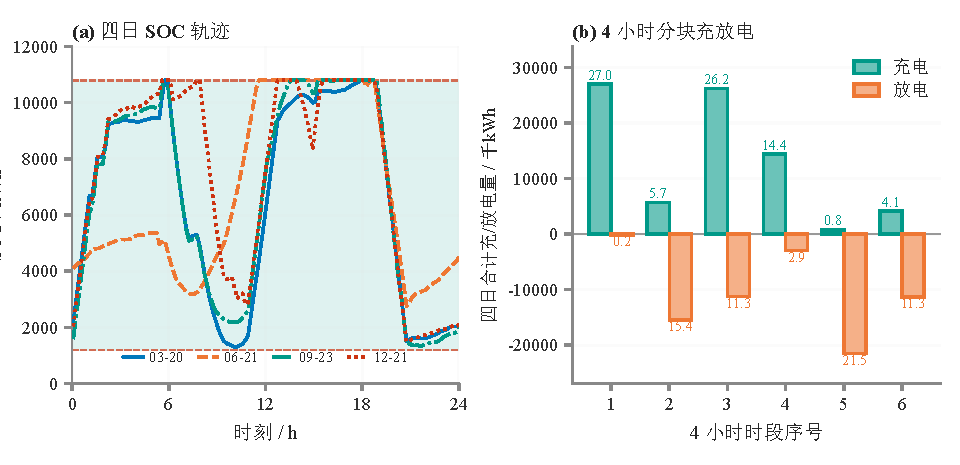
\includegraphics[width=0.85\textwidth]{figures/fig_p3_soc_4days.pdf}
  \caption{四指定日储能运行。(a) 四日 SOC 轨迹始终落在 1200--10\,800 kWh 安全边界内（虚线）；(b) 四日合计的分时段充放电呈“夜间充电、傍晚放电”的日内节律（第 1、3 时段充电约 27.0/26.2 千kWh，第 5 时段放电约 21.5 千kWh）。数据源：\texttt{data/p3\_specified\_dates\_timeseries.csv}、\texttt{data/p3\_storage\_4h\_summary\_4days.csv}。}
  \label{fig:p3-soc-4days}
\end{figure}

\begin{figure}[htbp]
  \centering
  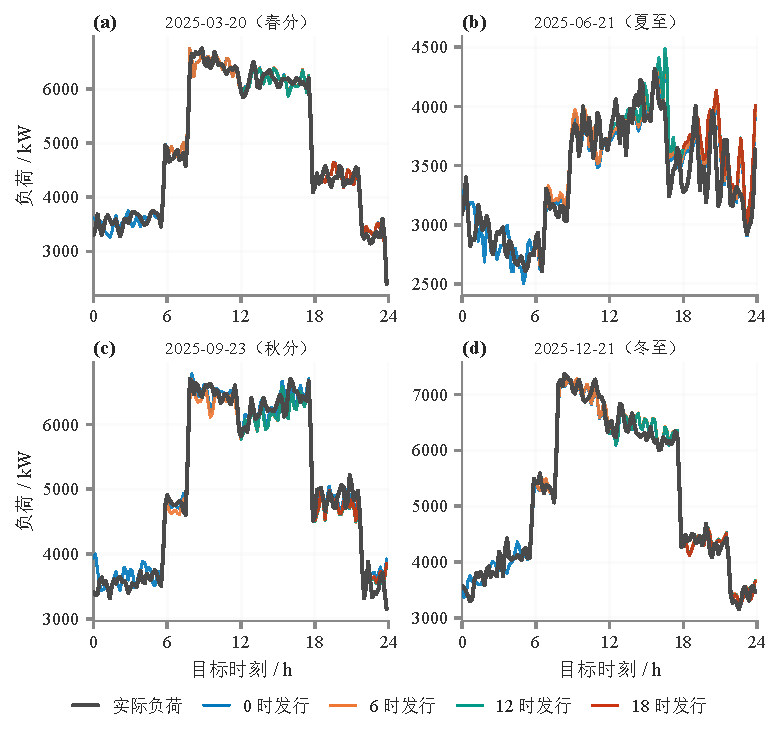
\includegraphics[width=0.70\textwidth]{figures/fig_p3_forecast_update.pdf}
  \caption{四个指定日 0/6/12/18 时发行的负荷预报与实际负荷。(a)--(d) 每个发行时刻只覆盖当天剩余时段，发行越晚覆盖越短且越贴近实际；同日曲线基本重合，说明新发行对负荷先验的修正有限，是否调整取决于 KEEP/ADJUST 判定而非曲线变化本身。数据源：\texttt{data/p3\_forecast\_specified\_dates.csv}。}
  \label{fig:p3-forecast-update}
\end{figure}

\begin{figure}[htbp]
  \centering
  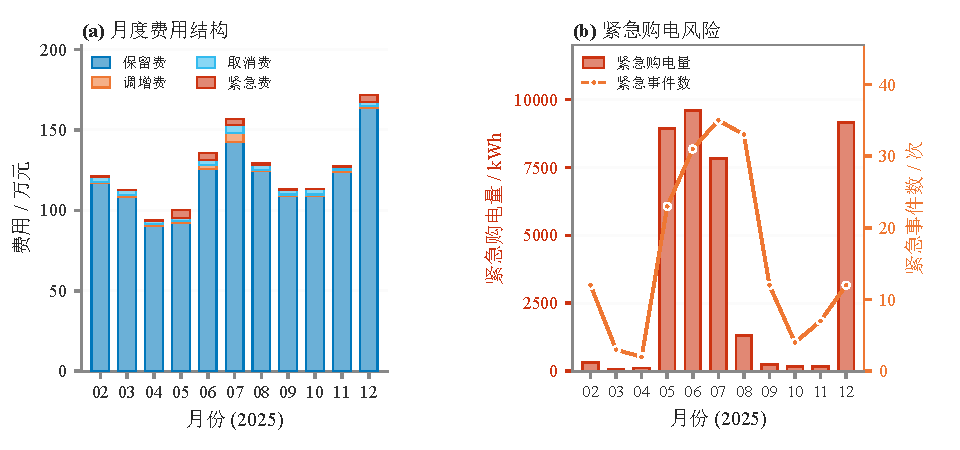
\includegraphics[width=0.85\textwidth]{figures/fig_p3_monthly_cost.pdf}
  \caption{MAIN 月度费用与紧急购电风险。(a) 月度费用按保留/调增/取消/紧急四分项堆叠，保留费主导账单；(b) 紧急购电集中出现在 5--7 月与 12 月（峰值 6 月约 9\,601 kWh，7 月 35 次事件）。全年总费用 1374.18 万元、紧急费 18.59 万元。数据源：\texttt{data/p3\_monthly\_cost\_summary\_MAIN.csv}。}
  \label{fig:p3-monthly-cost}
\end{figure}

% ---- 技术路线图 ----
\begin{figure}[htbp]
  \centering
  
\includegraphics[width=0.9\textwidth,height=0.72\textheight,keepaspectratio]{figures/fig_roadmap.pdf}
  \caption{Problem 3 整体技术路线图。五阶段：W1 周同期负荷基线 $\to$ 当天已完成前缀的低维收缩修正（次日不继承）$\to$ 附件3 官方 PV 与配对历史残差情景 $\to$ 0/6/12/18 向前 24h 滚动 LP 与同信息 KEEP/ADJUST 回放（$V_{\mathrm{score}}>0$ 才采纳）$\to$ 当前真实 SOC 逐10min 执行并按“保留1$p$/调增1.5$p$/取消0.5$p$/紧急5$p$”相对 $g^0$ 结算。可编辑源：\texttt{figures/fig\_roadmap.drawio}。}
  \label{fig:p3-roadmap}
\end{figure}
